\section{Basic Concepts}

In this course, we introduce numerical methods for the solution of \textbf{Partial Differential Equations} (PDEs), with focus on the \textbf{Finite Element} (FE) \textbf{method}\footnote{The \definition{Finite Element Method (FEM)}\label{definition: Finite Element Method (FEM)} is a popular method for numerically solving differential equations arising in engineering and mathematical modeling. Typical problem areas of interest include the traditional fields of structural analysis, heat transfer, fluid flow, mass transport, and electromagnetic potential. Computers are usually used to perform the calculations required. With high-speed supercomputers, better solutions can be achieved, and are often required to solve the largest and most complex problems. (\href{https://en.wikipedia.org/wiki/Finite_element_method}{source})} and the use of the computer for the construction of the PDEs numerical solution.

\highspace
We will consider the numerical approximation of elliptic and parabolic PDEs by considering their variational formulation, Galërkin and FE approximations in 1D/2D/3D, the theoretical properties and practical use of the methods, algorithmic aspects, and interpretation of the numerical results.

\highspace
Advanced topics include the approximation of saddle-point PDEs (Stokes equations), vectorial, nonlinear, and multiphysics differential problems, domain decomposition methods exploiting the properties of the PDEs, and the introduction to parallel computing for the FE method, i.e., in the \emph{High Performance Computing} (HPC) framework.

\highspace
Finally, the course will feature the use of the \href{https://www.dealii.org/}{\texttt{deal.II} software library}, a C++ open source FE library, and \href{https://www.paraview.org/}{ParaView} for the visualization of numerical solution and scientific computing data.

\newpage

\subsection{Mathematical Models and Scientific Computing}

\begin{definitionbox}[: Mathematical Model]
    A \definition{Mathematical Model} is a \textbf{set of} (algebraic or differential) \textbf{equations that is able to represent the features of a complex system or process}.

    \begin{flushleft}
        \textcolor{Green3}{\faIcon{question-circle} \textbf{Why do they exist?}}
    \end{flushleft}
    Models are \textbf{developed} to:
    \begin{itemize}
        \item Describe
        \item Forecast
        \item Control
    \end{itemize}
    The \textbf{behavior or evolution of such systems}.
\end{definitionbox}

\highspace
We are interested in the physics models. \textbf{Physics-based models} are those \textbf{mathematical models that are derived from physical principles} (like conservation laws of mass, momentum, energy, etc.) \textbf{and that encode natural laws of leading to (differential) equations whose solutions are often represented in the form of functions}. However, the analytical solution of such models is rarely available in closed form, for which numerical approximation methods are instead employed.

\highspace
\begin{definitionbox}[: Numerical Modelling]
    \definition{Numerical Modelling} indicates \textbf{sets of numerical methods that determine an approximate solution of the original} (often infinite-dimensional) \textbf{mathematical model}, by turing it into a \emph{discrete problem} (algebraic, finite-dimensional), whose dimension (size) is typically very large.
\end{definitionbox}

\highspace
\begin{definitionbox}[: Scientific Computing]
    \definition{Scientific Computing} is \textbf{a branch} of Mathematics \textbf{that numerically solves} (differential) \textbf{mathematical models by building approximate solutions though the use of a calculator}.
\end{definitionbox}

\highspace
For numerical models of large size, parallel architectures for calculators and the HPC framework are typically used.

\newpage

\begin{flushleft}
    \textcolor{Green3}{\faIcon{question-circle} \textbf{Why did we introduce mathematical models and physical models?}}
\end{flushleft}
Because they are connected and used together. Mathematical models are conventionally used altogether with theoretical (mathematical) models and experimental tests. Unfortunately, in several cases theoretical models are not available (like in Computational Medicine) or experimental tests are not meaningful or cannot be performed (for example, for nuclear testing). Physics-based models have witnessed an increasing role in the modern society in virtue of the massive developments of Scientific Computing and computational tools.

\highspace
Since a large amount of data is becoming available from multiple sources nowadays, data-driven models are fundamentals. \textbf{Data-driven models} are those mathematical models built from meaningful data that do not rely on physical principles, because the latter are not available or are not reliable, and whose construction calls for statical learning methods.

\highspace
Physics-based mathematical models (\textbf{mathematical problems}) are a fundamental pillar in the understanding and prediction of several physical phenomena and processes (\textbf{physical problems}). However, these mathematical models lead to problems that can rarely be solved analytically, or in an exact way (\textbf{exact solution}), especially for PDEs: with only a few exceptions, it is not possible to write their solution explicitly.

\highspace
Numerical methods and numerical approximation techniques (\textbf{numerical problems}) serve the purpose to determine an \textbf{approximate solution} of a mathematical model. When the calculator is used to determine such approximate solution, the latter is called \textbf{numerical solution} (see the Figure \ref{fig: scientific computing}).

\begin{figure}[!htp]
    \centering
    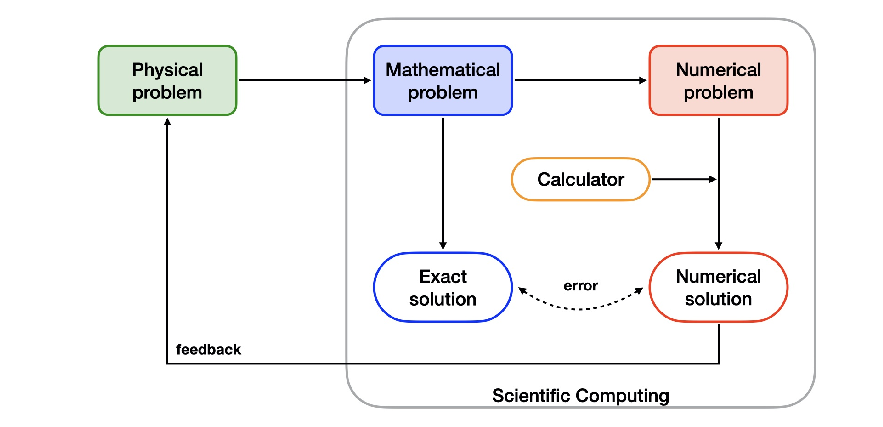
\includegraphics[width=\textwidth]{img/models-1.pdf}
    \caption{Scientific Computing.}
    \label{fig: scientific computing}
\end{figure}